\documentclass[12pt,fleqn]{article}\usepackage{../common}
\begin{document}


$$ 
c = \frac{ 2c_m}{1 + \cosh |b_c(t-t_{mc})|   }
$$


\begin{minted}[fontsize=\footnotesize]{python}
from scipy.optimize import fmin
import pandas as pd
#df = pd.read_csv('us.csv',sep='\s'); df['oil'] = df['oil'] / 1000.
df = pd.read_csv('world.csv',sep='\s')
#df = df[df['year'] < 1966]
#df = df[df['year'] < 2008]

def hubbard_err(w):
    cm=w[0];bc=w[1];tmc=w[2]
    #cm=2;bc=2;tmc=w[2]
    yfit = 2*cm / (1+cosh(bc*(df['year']-tmc)))
    diff = df['oil']-yfit
    e=norm(diff)
    return e

v = fmin(hubbard_err, [3, 3, 1900], maxiter=1000, maxfun=10000)
print v
df2 = df.set_index('year')
\end{minted}

\begin{verbatim}
Optimization terminated successfully.
         Current function value: 458.894642
         Iterations: 113
         Function evaluations: 222
[  3.22726098e+00  -1.26167397e-04   2.01249010e+03]
\end{verbatim}

\begin{minted}[fontsize=\footnotesize]{python}
ax = df2['oil'].plot(title='World Oil Production')
ax.set_ylabel("Barrels (Million)")
plt.savefig('peak_01.png')
\end{minted}


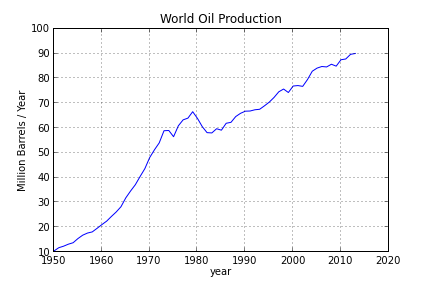
\includegraphics[height=6cm]{peak_01.png}

\begin{minted}[fontsize=\footnotesize]{python}
cm=v[0];bc=v[1];tmc=v[2]
#cm=2;bc=2;tmc=v[2]
def hubbard(x): return 2*cm / (1+cosh(bc*(x-tmc)))
pred = map(hubbard, df['year'])
print pred
df2['pred'] = pred
\end{minted}

\begin{verbatim}
[3.2272108284777965, 3.2272124207300186, 3.2272139872976742, 3.2272155281807131, 3.2272170433790874, 3.2272185328927483, 3.2272199967216486, 3.2272214348657418, 3.227222847324982, 3.2272242340993236, 3.227225595188723, 3.2272269305931371, 3.2272282403125221, 3.2272295243468387, 3.227230782696044, 3.2272320153600984, 3.2272332223389633, 3.2272344036325995, 3.2272355592409694, 3.2272366891640369, 3.2272377934017662, 3.2272388719541207, 3.2272399248210668, 3.227240952002572, 3.2272419534986021, 3.227242929309126, 3.2272438794341123, 3.2272448038735306, 3.2272457026273527, 3.2272465756955486, 3.227247423078091, 3.2272482447749526, 3.2272490407861079, 3.2272498111115313, 3.2272505557511981, 3.2272512747050848, 3.2272519679731673, 3.2272526355554261, 3.2272532774518377, 3.2272538936623825, 3.227254484187041, 3.2272550490257941, 3.2272555881786236, 3.227256101645513, 3.227256589426446, 3.2272570515214061, 3.2272574879303799, 3.227257898653352, 3.2272582836903099, 3.227258643041242, 3.2272589767061368, 3.2272592846849828, 3.2272595669777702, 3.2272598235844909, 3.2272600545051371, 3.2272602597396998, 3.2272604392881736, 3.2272605931505525, 3.227260721326831, 3.227260823817006, 3.2272609006210744, 3.2272609517390327, 3.22726097717088, 3.2272609769166154]
\end{verbatim}

\begin{minted}[fontsize=\footnotesize]{python}
ax = df2['oil'].plot(title='World Oil Production')
ax.set_ylabel("Barrels (Million)")
ax.hold(True)
ax = df2['pred'].plot()
plt.savefig('peak_02.png')
\end{minted}

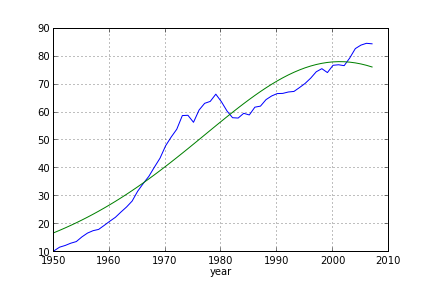
\includegraphics[height=6cm]{peak_02.png}

\url{http://www.earth-policy.org/Updates/2007/Update67_data2.htm#table1}

\url{http://en.wikipedia.org/wiki/Hubbert_curve}

\url{http://www.eia.gov/cfapps/ipdbproject/iedindex3.cfm?tid=5&pid=53&aid=1&cid=ww,&syid=1980&eyid=2013&unit=TBPD}

\url{http://www.countercurrents.org/mushalik270314.htm}

\url{http://www.eia.gov/dnav/pet/hist/LeafHandler.ashx?n=PET&s=MCRFPUS1&f=A}

\end{document}
